\documentclass[10pt]{article}
\usepackage{fancyhdr}
\usepackage{listings}
\usepackage{framed}
\usepackage{multicol}
\usepackage{tikz}
\usetikzlibrary{decorations.pathreplacing,shapes,arrows,positioning}

\setlength{\textwidth}{7.25in}
\setlength{\textheight}{9in}
\setlength{\topmargin}{-0.75in}
\setlength{\oddsidemargin}{-0.5in}
\setlength{\evensidemargin}{-0.5in}
\setlength{\headheight}{47pt}

\setlength\parindent{0pt}

\fancyhead[R]{CS 111C Jessica Masters\\
				Homework 6\\
				Chapter 11-13: Sorting\\
				Richard Szeto}
				
\pagestyle{fancy}

\lstset{language=Java}

\begin{document}
	\begin{center}
		\textbf{\large{Homework 6\\Chapter 11-13: Sorting}}
	\end{center}
	
	\section{Part I: Sort Traces}
		\begin{enumerate}
			\item Trace the sorts of the following dataset by hand using the six sorts listed below. Show the array each time it is altered.
				
				\vspace{0.5cm}
				Dataset:
				
				\begin{tikzpicture}
					\foreach \i [count=\n] in  
        			{6,8,3,10,9,6,7,1} 
           			\node[draw,minimum height=1cm,minimum width = 1cm,xshift=\n*1cm,font=\ttfamily](N\n){\i};
           		\end{tikzpicture}
           		
           		\vspace{0.5cm}
           		Note: I skip steps in the following algorithms when no changes are made to the array
           		
           		\vspace{0.5cm}
           		Sorts to trace:
           		
           		\begin{enumerate}
           			\item Selection sort
           				\begin{enumerate}           						
           					\item ~
           					
           						\begin{tikzpicture}
									\foreach \i [count=\n] in  
        							{6,8,3,10,9,6,7,1} 
           							\node[draw,minimum height=1cm,minimum width = 1cm,xshift=\n*1cm,font=\ttfamily](N\n){\i};
           							
           							\path[<->,>=stealth',thick]
           								(N1.north) edge [bend left] node {} (N8.north);
           							
           							\draw [decoration={brace,mirror,raise=5pt},decorate] (N1.south west) --  node[below=5pt]{\texttt{unsorted}}(N8.south east);
           						\end{tikzpicture}
           				
           					\item ~
           					
           						\begin{tikzpicture}
									\foreach \i [count=\n] in  
        							{1,8,3,10,9,6,7,6} 
           							\node[draw,minimum height=1cm,minimum width = 1cm,xshift=\n*1cm,font=\ttfamily](N\n){\i};          
           							
           							\path[<->,>=stealth',thick]
           								(N2.north) edge [bend left] node {} (N3.north); 							
           							
           							\draw [decoration={brace,mirror,raise=5pt},decorate] (N1.south west) --  node[below=5pt]{\texttt{sorted}}(N1.south east);
           							
           							\draw [decoration={brace,mirror,raise=5pt},decorate] (N2.south west) --  node[below=5pt]{\texttt{unsorted}}(N8.south east);
           						\end{tikzpicture}
           				
           					\item ~     
           					      					
           						\begin{tikzpicture}
									\foreach \i [count=\n] in  
        							{1,3,8,10,9,6,7,6} 
           							\node[draw,minimum height=1cm,minimum width = 1cm,xshift=\n*1cm,font=\ttfamily](N\n){\i};
           							
           							\path[<->,>=stealth',thick]
           								(N3.north) edge [bend left] node {} (N6.north);
           							
           							\draw [decoration={brace,mirror,raise=5pt},decorate] (N1.south west) --  node[below=5pt]{\texttt{sorted}}(N2.south east);
           							
           							\draw [decoration={brace,mirror,raise=5pt},decorate] (N3.south west) --  node[below=5pt]{\texttt{unsorted}}(N8.south east);
           						\end{tikzpicture}
           				
           					\item ~   
           					        					
           						\begin{tikzpicture}
									\foreach \i [count=\n] in  
        							{1,3,6,10,9,8,7,6} 
           							\node[draw,minimum height=1cm,minimum width = 1cm,xshift=\n*1cm,font=\ttfamily](N\n){\i};
           							
           							\path[<->,>=stealth',thick]
           								(N4.north) edge [bend left] node {} (N8.north);
           							
           							\draw [decoration={brace,mirror,raise=5pt},decorate] (N1.south west) --  node[below=5pt]{\texttt{sorted}}(N3.south east);
           							
           							\draw [decoration={brace,mirror,raise=5pt},decorate] (N4.south west) --  node[below=5pt]{\texttt{unsorted}}(N8.south east);
           						\end{tikzpicture}
           				
           					\item ~         
           					  					
           						\begin{tikzpicture}
									\foreach \i [count=\n] in  
        							{1,3,6,6,9,8,7,10} 
           							\node[draw,minimum height=1cm,minimum width = 1cm,xshift=\n*1cm,font=\ttfamily](N\n){\i};
           							
           							\path[<->,>=stealth',thick]
           								(N5.north) edge [bend left] node {} (N7.north);
           							
           							\draw [decoration={brace,mirror,raise=5pt},decorate] (N1.south west) --  node[below=5pt]{\texttt{sorted}}(N4.south east);
           							
           							\draw [decoration={brace,mirror,raise=5pt},decorate] (N5.south west) --  node[below=5pt]{\texttt{unsorted}}(N8.south east);
           						\end{tikzpicture}
           					
           					\item ~
           						
           						\begin{tikzpicture}
									\foreach \i [count=\n] in  
        							{1,3,6,6,7,8,9,10} 
           							\node[draw,minimum height=1cm,minimum width = 1cm,xshift=\n*1cm,font=\ttfamily](N\n){\i};
           							
           							\draw [decoration={brace,mirror,raise=5pt},decorate] (N1.south west) --  node[below=5pt]{\texttt{sorted}}(N8.south east);
           						\end{tikzpicture}
           				\end{enumerate}
           			
           			\item Insertion sort
           				\begin{enumerate}
           						
           					\item ~
           					
           						\begin{tikzpicture}
									\foreach \i [count=\n] in  
        							{6,8,3,10,9,6,7,1} 
           							\node[draw,minimum height=1cm,minimum width = 1cm,xshift=\n*1cm,font=\ttfamily](N\n){\i};
           							
           							\draw [decoration={brace,mirror,raise=5pt},decorate] (N1.south west) --  node[below=5pt]{\texttt{sorted}}(N2.south east);
           							
           							\draw [decoration={brace,mirror,raise=5pt},decorate] (N3.south west) --  node[below=5pt]{\texttt{unsorted}}(N8.south east);
           						\end{tikzpicture}
           						
           					\item ~
           					
           						\begin{tikzpicture}
									\foreach \i [count=\n] in  
        							{6,8,,10,9,6,7,1} 
           							\node[draw,minimum height=1cm,minimum width = 1cm,xshift=\n*1cm,font=\ttfamily](N\n){\i};
           							
           							\draw (N3.south) -- node[draw,minimum height=1cm,minimum width=1cm,yshift=-1cm,font=\ttfamily](N9){3}(N3.south); 
           							
           							\path[->,>=stealth',thick]
           								(N3.south) edge node {} (N9.north)
           								(N9.west) edge [bend left] node {} (N1.south);
           							
           							\foreach \i in {1,2}
           							{
           								\pgfmathtruncatemacro{\TempVar}{\i+1}
           								
           								\path[->,>=stealth',thick]
           									(N\i.north) edge [bend left] node {} (N\TempVar.north);
           							}
           						\end{tikzpicture}
           						
           						\vspace{0.5cm}
           						\begin{tikzpicture}
									\foreach \i [count=\n] in  
        							{3,6,8,10,9,6,7,1} 
           							\node[draw,minimum height=1cm,minimum width = 1cm,xshift=\n*1cm,font=\ttfamily](N\n){\i};
           							
           							\draw [decoration={brace,mirror,raise=5pt},decorate] (N1.south west) --  node[below=5pt]{\texttt{sorted}}(N4.south east);
           							
           							\draw [decoration={brace,mirror,raise=5pt},decorate] (N5.south west) --  node[below=5pt]{\texttt{unsorted}}(N8.south east);
           						\end{tikzpicture}
           					
           					\item ~
           						
           						\begin{tikzpicture}
									\foreach \i [count=\n] in  
        							{3,6,8,10,,6,7,1} 
           							\node[draw,minimum height=1cm,minimum width = 1cm,xshift=\n*1cm,font=\ttfamily](N\n){\i};
           							
           							\draw (N5.south) -- node[draw,minimum height=1cm,minimum width=1cm,yshift=-1cm,font=\ttfamily](N9){9}(N5.south); 
           							
           							\path[->,>=stealth',thick]
           								(N5.south) edge node {} (N9.north)
           								(N4.north) edge [bend left] node {} (N5.north)
           								(N9.west) edge [bend left] node {} (N4.south);
           						\end{tikzpicture}
           						
           						\vspace{0.5cm}
           						\begin{tikzpicture}
									\foreach \i [count=\n] in  
        							{3,6,8,9,10,6,7,1} 
           							\node[draw,minimum height=1cm,minimum width = 1cm,xshift=\n*1cm,font=\ttfamily](N\n){\i};
           							
           							\draw [decoration={brace,mirror,raise=5pt},decorate] (N1.south west) --  node[below=5pt]{\texttt{sorted}}(N5.south east);
           							
           							\draw [decoration={brace,mirror,raise=5pt},decorate] (N6.south west) --  node[below=5pt]{\texttt{unsorted}}(N8.south east);
           						\end{tikzpicture}
           					
           					\item ~
           						
           						\begin{tikzpicture}
									\foreach \i [count=\n] in  
        							{3,6,8,9,10,,7,1} 
           							\node[draw,minimum height=1cm,minimum width = 1cm,xshift=\n*1cm,font=\ttfamily](N\n){\i};
           							
           							\draw (N6.south) -- node[draw,minimum height=1cm,minimum width=1cm,yshift=-1cm,font=\ttfamily](N9){6}(N6.south); 
           							
           							\path[->,>=stealth',thick]
           								(N6.south) edge node {} (N9.north)
           								(N9.west) edge [bend left] node {} (N3.south);
           							
           							\foreach \i in {3,...,5}
           							{
           								\pgfmathtruncatemacro{\TempVar}{\i+1}
           								
           								\path[->,>=stealth',thick]
           									(N\i.north) edge [bend left] node {} (N\TempVar.north);
           							}
           						\end{tikzpicture}
           						
           						\vspace{0.5cm}
           						\begin{tikzpicture}
									\foreach \i [count=\n] in  
        							{3,6,6,8,9,10,7,1} 
           							\node[draw,minimum height=1cm,minimum width = 1cm,xshift=\n*1cm,font=\ttfamily](N\n){\i};
           							
           							\draw [decoration={brace,mirror,raise=5pt},decorate] (N1.south west) --  node[below=5pt]{\texttt{sorted}}(N6.south east);
           							
           							\draw [decoration={brace,mirror,raise=5pt},decorate] (N7.south west) --  node[below=5pt]{\texttt{unsorted}}(N8.south east);
           						\end{tikzpicture}
           					
           					\item ~
           						
           						\begin{tikzpicture}
									\foreach \i [count=\n] in  
        							{3,6,6,8,9,10,,1} 
           							\node[draw,minimum height=1cm,minimum width = 1cm,xshift=\n*1cm,font=\ttfamily](N\n){\i};
           							
           							\draw (N7.south) -- node[draw,minimum height=1cm,minimum width=1cm,yshift=-1cm,font=\ttfamily](N9){7}(N7.south); 
           							
           							\path[->,>=stealth',thick]
           								(N7.south) edge node {} (N9.north)
           								(N9.west) edge [bend left] node {} (N4.south);
           							
           							\foreach \i in {4,...,6}
           							{
           								\pgfmathtruncatemacro{\TempVar}{\i+1}
           								\path[->,>=stealth',thick]
           									(N\i.north) edge [bend left] node {} (N\TempVar.north);
           							}
           						\end{tikzpicture}
           						
           						\vspace{0.5cm}
           						\begin{tikzpicture}
									\foreach \i [count=\n] in  
        							{3,6,6,7,8,9,10,1} 
           							\node[draw,minimum height=1cm,minimum width = 1cm,xshift=\n*1cm,font=\ttfamily](N\n){\i};
           							
           							\draw [decoration={brace,mirror,raise=5pt},decorate] (N1.south west) --  node[below=5pt]{\texttt{sorted}}(N7.south east);
           							
           							\draw [decoration={brace,mirror,raise=5pt},decorate] (N8.south west) --  node[below=5pt]{\texttt{unsorted}}(N8.south east);
           						\end{tikzpicture}
           					
           					\item ~
           						
           						\begin{tikzpicture}
									\foreach \i [count=\n] in  
        							{3,6,6,7,8,9,10,} 
           							\node[draw,minimum height=1cm,minimum width = 1cm,xshift=\n*1cm,font=\ttfamily](N\n){\i};
           							
           							\draw (N8.south) -- node[draw,minimum height=1cm,minimum width=1cm,yshift=-1cm,font=\ttfamily](N9){1}(N8.south); 
           							
           							\path[->,>=stealth',thick]
           								(N8.south) edge node {} (N9.north)
           								(N9.west) edge [bend left] node {} (N1.south);
           								
           							\foreach \i in {1,...,7}
           							{
           								\pgfmathtruncatemacro{\TempVar}{\i+1}
           								\path[->,>=stealth',thick]
           									(N\i.north) edge [bend left] node {} (N\TempVar.north);
           							}
           						\end{tikzpicture}
           						
           						\vspace{0.5cm}
           						\begin{tikzpicture}
									\foreach \i [count=\n] in  
        							{1,3,6,6,7,8,9,10} 
           							\node[draw,minimum height=1cm,minimum width = 1cm,xshift=\n*1cm,font=\ttfamily](N\n){\i};
           							
           							\draw [decoration={brace,mirror,raise=5pt},decorate] (N1.south west) --  node[below=5pt]{\texttt{sorted}}(N8.south east);
           						\end{tikzpicture}
           				\end{enumerate}
           				
           			\item Shell sort
           				\begin{itemize}
           					\item In addition to showing the contents of the array, also list what the gap is for that part of the trace.
           				\end{itemize}
           				
           				\begin{enumerate}
           				
           					\item Space = 4
           						
           						\begin{tikzpicture}
									\foreach \i [count=\n] in {6,8,3,10,9,6,7,1} 
           								\node[draw,minimum height=1cm,minimum width = 1cm,xshift=\n*1cm,font=\ttfamily](N\n){\i};
           							
           							\draw [decoration={brace,mirror,raise=5pt},decorate] (N1.south) --  node[below=5pt]{\texttt{subarray}}(N5.south);
           						\end{tikzpicture}
           						
           						\vspace{0.5cm}
           						\begin{tikzpicture}
									\foreach \i [count=\n] in {6,8,3,10,9,,7,1} 
           								\node[draw,minimum height=1cm,minimum width = 1cm,xshift=\n*1cm,font=\ttfamily](N\n){\i};
           							
           							\draw [decoration={brace,mirror,raise=5pt},decorate] (N2.south) --  node[below=5pt]{\texttt{subarray}}(N6.south);
           							
           							\draw (N6.south) -- node[draw,minimum height=1cm,minimum width=1cm,yshift=-1cm,font=\ttfamily](N9){6}(N6.south);
           							
           							\path [->,>=stealth',thick]
           								(N6.south) edge node {} (N9.north)
           								(N2.north) edge [bend left] node {} (N6.north)
           								(N9.west) edge [bend left] node {} (N2.south);
           						\end{tikzpicture}
           						
           						\vspace{0.5cm}
           						\begin{tikzpicture}
									\foreach \i [count=\n] in {6,6,3,10,9,8,7,1} 
           								\node[draw,minimum height=1cm,minimum width = 1cm,xshift=\n*1cm,font=\ttfamily](N\n){\i};
           							
           							\draw [decoration={brace,mirror,raise=5pt},decorate] (N3.south) --  node[below=5pt]{\texttt{subarray}}(N7.south);
           						\end{tikzpicture}
           						
           						\vspace{0.5cm}
           						\begin{tikzpicture}
									\foreach \i [count=\n] in {6,6,3,10,9,8,7,} 
           								\node[draw,minimum height=1cm,minimum width = 1cm,xshift=\n*1cm,font=\ttfamily](N\n){\i};
           								
           							\draw [decoration={brace,mirror,raise=5pt},decorate] (N4.south) --  node[below=5pt]{\texttt{subarray}}(N8.south);
           							
           							\draw (N8.south) -- node[draw,minimum height=1cm,minimum width=1cm,yshift=-1cm,font=\ttfamily](N9){1}(N8.south);
           							
           							\path [->,>=stealth',thick]
           								(N8.south) edge node {} (N9.north)
           								(N4.north) edge [bend left] node {} (N8.north)
           								(N9.west) edge [bend left] node {} (N4.south);
           						\end{tikzpicture}
           						
           						\vspace{0.5cm}
           						\begin{tikzpicture}
									\foreach \i [count=\n] in {6,6,3,1,9,8,7,10} 
           								\node[draw,minimum height=1cm,minimum width = 1cm,xshift=\n*1cm,font=\ttfamily](N\n){\i};
           								
           							\draw [decoration={brace,mirror,raise=5pt},decorate] (N4.south) --  node[below=5pt]{\texttt{subarray}}(N8.south);
           						\end{tikzpicture}
           						
           					\item Space = 2
           						
           						\begin{tikzpicture}
									\foreach \i [count=\n] in {6,6,,1,9,8,7,10} 
           								\node[draw,minimum height=1cm,minimum width = 1cm,xshift=\n*1cm,font=\ttfamily](N\n){\i};
           								
           							\draw [decoration={brace,mirror,raise=5pt},decorate] (N1.south) --  node[below=5pt]{\texttt{subarray}}(N3.south);
           							
           							\draw [decoration={brace,mirror,raise=5pt},decorate] (N3.south) --  node[below=5pt]{\texttt{subarray}}(N5.south);
           							
           							\draw [decoration={brace,mirror,raise=5pt},decorate] (N5.south) --  node[below=5pt]{\texttt{subarray}}(N7.south);
           							
           							\draw (N3.south) -- node[draw,minimum height=1cm,minimum width=1cm,yshift=-1cm,font=\ttfamily](N9){3}(N3.south);
           							
           							\path [->,>=stealth',thick]
           								(N3.south) edge node {} (N9.north)
           								(N1.north) edge [bend left] node {} (N3.north)
           								(N9.west) edge [bend left] node {} (N1.south);
           						\end{tikzpicture}
           						
           						\vspace{0.5cm}
           						\begin{tikzpicture}
									\foreach \i [count=\n] in {3,6,6,1,9,8,,10} 
           								\node[draw,minimum height=1cm,minimum width = 1cm,xshift=\n*1cm,font=\ttfamily](N\n){\i};
           								
           							\draw [decoration={brace,mirror,raise=5pt},decorate] (N1.south) --  node[below=5pt]{\texttt{subarray}}(N3.south);
           							
           							\draw [decoration={brace,mirror,raise=5pt},decorate] (N3.south) --  node[below=5pt]{\texttt{subarray}}(N5.south);
           							
           							\draw [decoration={brace,mirror,raise=5pt},decorate] (N5.south) --  node[below=5pt]{\texttt{subarray}}(N7.south);
           							
           							\draw (N7.south) -- node[draw,minimum height=1cm,minimum width=1cm,yshift=-1cm,font=\ttfamily](N9){7}(N7.south);
           							
           							\path [->,>=stealth',thick]
           								(N7.south) edge node {} (N9.north)
           								(N5.north) edge [bend left] node {} (N7.north)
           								(N9.west) edge [bend left] node {} (N5.south);
           						\end{tikzpicture}
           						
           						\vspace{0.5cm}
           						\begin{tikzpicture}
									\foreach \i [count=\n] in {3,6,6,,7,8,9,10} 
           								\node[draw,minimum height=1cm,minimum width = 1cm,xshift=\n*1cm,font=\ttfamily](N\n){\i};
           								
           							\draw [decoration={brace,mirror,raise=5pt},decorate] (N2.south) --  node[below=5pt]{\texttt{subarray}}(N4.south);
           							
           							\draw [decoration={brace,mirror,raise=5pt},decorate] (N4.south) --  node[below=5pt]{\texttt{subarray}}(N6.south);
           							
           							\draw [decoration={brace,mirror,raise=5pt},decorate] (N6.south) --  node[below=5pt]{\texttt{subarray}}(N8.south);
           							
           							\draw (N4.south) -- node[draw,minimum height=1cm,minimum width=1cm,yshift=-1cm,font=\ttfamily](N9){1}(N4.south);
           							
           							\path [->,>=stealth',thick]
           								(N4.south) edge node {} (N9.north)
           								(N2.north) edge [bend left] node {} (N4.north)
           								(N9.west) edge [bend left] node {} (N2.south);
           						\end{tikzpicture}
           						
           						\vspace{0.5cm}
           						\begin{tikzpicture}
									\foreach \i [count=\n] in {3,1,6,6,7,8,9,10} 
           								\node[draw,minimum height=1cm,minimum width = 1cm,xshift=\n*1cm,font=\ttfamily](N\n){\i};
           								
           							\draw [decoration={brace,mirror,raise=5pt},decorate] (N2.south) --  node[below=5pt]{\texttt{subarray}}(N4.south);
           							
           							\draw [decoration={brace,mirror,raise=5pt},decorate] (N4.south) --  node[below=5pt]{\texttt{subarray}}(N6.south);
           							
           							\draw [decoration={brace,mirror,raise=5pt},decorate] (N6.south) --  node[below=5pt]{\texttt{subarray}}(N8.south);
           						\end{tikzpicture}
           					
           					\item Space = 1
           						
           						\begin{tikzpicture}
									\foreach \i [count=\n] in {3,,6,6,7,8,9,10} 
           								\node[draw,minimum height=1cm,minimum width = 1cm,xshift=\n*1cm,font=\ttfamily](N\n){\i};
           								
           							\draw (N2.south) -- node[draw,minimum height=1cm,minimum width=1cm,yshift=-1cm,font=\ttfamily](N9){1}(N2.south);
           							
           							\path [->,>=stealth',thick]
           								(N2.south) edge node {} (N9.north)
           								(N1.north) edge [bend left] node {} (N2.north)
           								(N9.west) edge [bend left] node {} (N1.south);
           						\end{tikzpicture}
           						
           						\vspace{0.5cm}
           						\begin{tikzpicture}
									\foreach \i [count=\n] in {1,3,6,6,7,8,9,10} 
           								\node[draw,minimum height=1cm,minimum width = 1cm,xshift=\n*1cm,font=\ttfamily](N\n){\i};
           						\end{tikzpicture}
           				
           				\end{enumerate}
           			
           			\item Merge sort
           				
           				\begin{enumerate}          					
           					\item Recursively split the array in half until we have two subarrays where they are both length = 1
           						
           						\vspace{0.5cm}
           						\begin{tikzpicture}
									\foreach \i [count=\n] in {6,8,3,10,9,6,7,1} 
           								\node[draw,minimum height=1cm,minimum width = 1cm,xshift=4.5cm+\n*1cm,font=\ttfamily](A\n){\i};
           							
           							\node[draw,circle,minimum height = 0.5cm,xshift=4.5cm,minimum width = 0.5cm](A9){1};
           						
									\foreach \i [count=\n] in {6,8,3,10} 
           								\node[draw,minimum height=1cm,minimum width = 1cm,xshift=2.5cm+\n*1cm,yshift=-1.5cm,font=\ttfamily](B\n){\i};
           								
           							\node[draw,circle,minimum height = 0.5cm,xshift=2.5cm,yshift=-1.5cm,minimum width = 0.5cm](B4){2};
           								
           							\foreach \i [count=\n] in {9,6,7,1}
           								\node[draw,minimum height=1cm,minimum width = 1cm,xshift=10.5cm+\n*1cm,yshift=-1.5cm,font=\ttfamily](C\n){\i};
           							
           							\node[draw,circle,minimum height = 0.5cm,xshift=10.5cm,yshift=-1.5cm,minimum width = 0.5cm](C5){12};

									\foreach \i [count=\n] in {6,8} 
           								\node[draw,minimum height=1cm,minimum width = 1cm,xshift=1.5cm+\n*1cm,yshift=-3cm,font=\ttfamily](D\n){\i};
           							
           							\node[draw,circle,minimum height = 0.5cm,xshift=1.5cm,yshift=-3cm,minimum width = 0.5cm](D3){3};
           								
           							\foreach \i [count=\n] in {3,10}
           								\node[draw,minimum height=1cm,minimum width = 1cm,xshift=5.5cm+\n*1cm,yshift=-3cm,font=\ttfamily](E\n){\i};
           							
           							\node[draw,circle,minimum height = 0.5cm,xshift=5.5cm,yshift=-3cm,minimum width = 0.5cm](E3){7};
           								
           							\foreach \i [count=\n] in {9,6}
           								\node[draw,minimum height=1cm,minimum width = 1cm,xshift=9.5cm+\n*1cm,yshift=-3cm,font=\ttfamily](F\n){\i};
           							
           							\node[draw,circle,minimum height = 0.5cm,xshift=9.5cm,yshift=-3cm,minimum width = 0.5cm](F3){13};
           								
           							\foreach \i [count=\n] in {7,1}
           								\node[draw,minimum height=1cm,minimum width = 1cm,xshift=13.5cm+\n*1cm,yshift=-3cm,font=\ttfamily](G\n){\i};
           							
           							\node[draw,circle,minimum height = 0.5cm,xshift=13.5cm,yshift=-3cm,minimum width = 0.5cm](G3){17};

									\foreach \i [count=\n] in {6,8,3,10,9,6,7,1} 
           								\node[draw,minimum height=1cm,minimum width = 1cm,xshift=\n*2cm,yshift=-4.5cm,font=\ttfamily](H\n){\i};
           							
           							\node[draw,circle,minimum height = 0.5cm,xshift=1cm,yshift=-4.5cm,minimum width = 0.5cm](H9){4};
           							
           							\node[draw,circle,minimum height = 0.5cm,xshift=3cm,yshift=-4.5cm,minimum width = 0.5cm](H10){5};
           							
           							\node[draw,circle,minimum height = 0.5cm,xshift=5cm,yshift=-4.5cm,minimum width = 0.5cm](H11){8};
           							
           							\node[draw,circle,minimum height = 0.5cm,xshift=7cm,yshift=-4.5cm,minimum width = 0.5cm](H12){9};
           							
           							\node[draw,circle,minimum height = 0.5cm,xshift=9cm,yshift=-4.5cm,minimum width = 0.5cm](H13){14};
           							
           							\node[draw,circle,minimum height = 0.5cm,xshift=11cm,yshift=-4.5cm,minimum width = 0.5cm](H14){15};
           							
           							\node[draw,circle,minimum height = 0.5cm,xshift=13cm,yshift=-4.5cm,minimum width = 0.5cm](H15){18};
           							
           							\node[draw,circle,minimum height = 0.5cm,xshift=15cm,yshift=-4.5cm,minimum width = 0.5cm](H16){19};
           								
           							\path [->,>=stealth',thick]
           								(A2.south east) edge node {} (B2.north east)
           								(A6.south east) edge node {} (C2.north east)
           								(B1.south east) edge node {} (D1.north east)
           								(B3.south east) edge node {} (E1.north east)
           								(C1.south east) edge node {} (F1.north east)
           								(C3.south east) edge node {} (G1.north east)
           								(D1.south) edge node {} (H1.north)
           								(D2.south) edge node {} (H2.north)
           								(E1.south) edge node {} (H3.north)
           								(E2.south) edge node {} (H4.north)
           								(F1.south) edge node {} (H5.north)
           								(F2.south) edge node {} (H6.north)
           								(G1.south) edge node {} (H7.north)
           								(G2.south) edge node {} (H8.north);
           						\end{tikzpicture}
           					
           					\item sort and merge
           						
           						\vspace{0.5cm}
           						\begin{tikzpicture}
           							\foreach \i [count=\n] in {6,8,3,10,9,6,7,1} 
           								\node[draw,minimum height=1cm,minimum width = 1cm,xshift=\n*2cm,font=\ttfamily](H\n){\i};
           							
           							\node[circle,minimum height = 0.6cm,xshift=1cm,minimum width = 0.6cm](H9){};
           								
           							\foreach \i [count=\n] in {6,8} 
           								\node[draw,minimum height=1cm,minimum width = 1cm,xshift=1.5cm+\n*1cm,yshift=-1.5cm,font=\ttfamily](D\n){\i};
           							
           							\node[draw,circle,minimum height = 0.5cm,xshift=1.5cm,yshift=-1.5cm,minimum width = 0.5cm](D3){6};
           								
           							\foreach \i [count=\n] in {3,10}
           								\node[draw,minimum height=1cm,minimum width = 1cm,xshift=5.5cm+\n*1cm,yshift=-1.5cm,font=\ttfamily](E\n){\i};
           							
           							\node[draw,circle,minimum height = 0.5cm,xshift=5.5cm,yshift=-1.5cm,minimum width = 0.5cm](E3){10};
           								
           							\foreach \i [count=\n] in {6,9}
           								\node[draw,minimum height=1cm,minimum width = 1cm,xshift=9.5cm+\n*1cm,yshift=-1.5cm,font=\ttfamily](F\n){\i};
           							
           							\node[draw,circle,minimum height = 0.5cm,xshift=9.5cm,yshift=-1.5cm,minimum width = 0.5cm](F3){16};
           								
           							\foreach \i [count=\n] in {1,7}
           								\node[draw,minimum height=1cm,minimum width = 1cm,xshift=13.5cm+\n*1cm,yshift=-1.5cm,font=\ttfamily](G\n){\i};
           							
           							\node[draw,circle,minimum height = 0.5cm,xshift=13.5cm,yshift=-1.5cm,minimum width = 0.5cm](G3){20};
           							
           							\foreach \i [count=\n] in {3,6,8,10} 
           								\node[draw,minimum height=1cm,minimum width = 1cm,xshift=2.5cm+\n*1cm,yshift=-4cm,font=\ttfamily](B\n){\i};
           								
           							\node[draw,circle,minimum height = 0.5cm,xshift=2.5cm,yshift=-4cm,minimum width = 0.5cm](B5){11};
           								
           							\foreach \i [count=\n] in {1,6,7,9}
           								\node[draw,minimum height=1cm,minimum width = 1cm,xshift=10.5cm+\n*1cm,yshift=-4cm,font=\ttfamily](C\n){\i};
           							
           							\node[draw,circle,minimum height = 0.5cm,xshift=10.5cm,yshift=-4cm,minimum width = 0.5cm](C5){21};
           								
           							\foreach \i [count=\n] in {1,3,6,6,7,8,9,10} 
           								\node[draw,minimum height=1cm,minimum width = 1cm,xshift=4.5cm+\n*1cm,yshift=-8cm,font=\ttfamily](A\n){\i};
           							
           							\node[draw,circle,minimum height = 0.5cm,xshift=4.5cm,yshift=-8cm,minimum width = 0.5cm](A9){22};
           							
           							\path [->,>=stealth',thick]
           								(H1.south) edge node {} (D1.north)
           								(H2.south) edge node {} (D2.north)
           								(H3.south) edge node {} (E1.north)
           								(H4.south) edge node {} (E2.north)
           								(H5.south) edge node {} (F2.north)
           								(H6.south) edge node {} (F1.north)
           								(H7.south) edge node {} (G2.north)
           								(H8.south) edge node {} (G1.north)
           								
           								(E1.south) edge node {} (B1.north)
           								(D1.south) edge node {} (B2.north)
           								(D2.south) edge node {} (B3.north)
           								(E2.south) edge node {} (B4.north)
           								
           								(G1.south) edge node {} (C1.north)
           								(F1.south) edge node {} (C2.north)
           								(G2.south) edge node {} (C3.north)
           								(F2.south) edge node {} (C4.north)
           								
           								(C1.south) edge node {} (A1.north)
           								(B1.south) edge node {} (A2.north)
           								(B2.south) edge node {} (A3.north)
           								(C2.south) edge node {} (A4.north)
           								(C3.south) edge node {} (A5.north)
           								(B3.south) edge node {} (A6.north)
           								(C4.south) edge node {} (A7.north)
           								(B4.south) edge node {} (A8.north);
           						\end{tikzpicture}
           						
           				\end{enumerate}
           			
           			\item Quick sort
           				\begin{itemize}
           					\item Use the code given in Section 18. I recommend writing out the variables to help with your trace (e.g., pivotIndex, pivot, indexFromLeft, etc.).
           					\item You only need to show the results after the first partition step. In other words, show how the array is changed after the first call to the partition method (displayed in Section 17). 
           					\item Also submit what the parameters will be for the next two recursive calls to quickSort
           				\end{itemize}
           				
           				\begin{enumerate}
           					\item Dataset:
           						
           						\begin{tikzpicture}
									\foreach \i [count=\n] in {6,8,3,10,9,6,7,1} 
           								\node[draw,minimum height=1cm,minimum width = 1cm,xshift=\n*1cm,font=\ttfamily](N\n){\i};
           						\end{tikzpicture}
           					
           					\item \texttt{quickSort(array,0,array.length - 1)}
           						
           						\begin{enumerate}
           							\item \texttt{pivotIndex = partition(array,0,7)}
           							
           								\begin{itemize}
           									\item \texttt{sortFirstMiddle(array,0,3,7)}
           										
           										\begin{tikzpicture}
													\foreach \i [count=\n] in {6,8,3,10,9,6,7,1} 
           												\node[draw,minimum height=1cm,minimum width = 1cm,xshift=\n*1cm,font=\ttfamily](N\n){\i};
           											
           											\draw [decoration={brace,mirror,raise=5pt},decorate] (N1.south west) --  node[below=5pt]{\texttt{first}}(N1.south east);
           											
           											\draw [decoration={brace,mirror,raise=5pt},decorate] (N4.south west) --  node[below=5pt]{\texttt{middle}}(N4.south east);
           											
           											\draw [decoration={brace,mirror,raise=5pt},decorate] (N8.south west) --  node[below=5pt]{\texttt{last}}(N8.south east);
           											
           											\path [<->,>=stealth',thick]
           												(N4.north) edge [bend left] node {} (N8.north);
           										\end{tikzpicture}
           										
           										\vspace{0.5cm}
           										\begin{tikzpicture}
													\foreach \i [count=\n] in {6,8,3,1,9,6,7,10} 
           												\node[draw,minimum height=1cm,minimum width = 1cm,xshift=\n*1cm,font=\ttfamily](N\n){\i};
           											
           											\draw [decoration={brace,mirror,raise=5pt},decorate] (N1.south west) --  node[below=5pt]{\texttt{first}}(N1.south east);
           											
           											\draw [decoration={brace,mirror,raise=5pt},decorate] (N4.south west) --  node[below=5pt]{\texttt{middle}}(N4.south east);
           											
           											\draw [decoration={brace,mirror,raise=5pt},decorate] (N8.south west) --  node[below=5pt]{\texttt{last}}(N8.south east);
           											
           											\path [<->,>=stealth',thick]
           												(N1.north) edge [bend left] node {} (N4.north);
           										\end{tikzpicture}
           										
           										\vspace{0.5cm}
           										\begin{tikzpicture}
													\foreach \i [count=\n] in {1,8,3,6,9,6,7,10} 
           												\node[draw,minimum height=1cm,minimum width = 1cm,xshift=\n*1cm,font=\ttfamily](N\n){\i};
           											
           											\draw [decoration={brace,mirror,raise=5pt},decorate] (N1.south west) --  node[below=5pt]{\texttt{first}}(N1.south east);
           											
           											\draw [decoration={brace,mirror,raise=5pt},decorate] (N4.south west) --  node[below=5pt]{\texttt{middle}}(N4.south east);
           											
           											\draw [decoration={brace,mirror,raise=5pt},decorate] (N8.south west) --  node[below=5pt]{\texttt{last}}(N8.south east);
           										\end{tikzpicture}
           									
           									\item \texttt{swap(array,mid,last-1)}
           									
           										\begin{tikzpicture}
													\foreach \i [count=\n] in {1,8,3,6,9,6,7,10} 
           												\node[draw,minimum height=1cm,minimum width = 1cm,xshift=\n*1cm,font=\ttfamily](N\n){\i};
           											
           											\draw [decoration={brace,mirror,raise=5pt},decorate] (N4.south west) --  node[below=5pt]{\texttt{mid}}(N4.south east);
           											
           											\draw [decoration={brace,mirror,raise=5pt},decorate] (N7.south west) --  node[below=5pt]{\texttt{last-1}}(N7.south east);
           								
           											\path [<->,>=stealth',thick]
           												(N4.north) edge [bend left] node {} (N7.north);
           										\end{tikzpicture}
           										
           										\vspace{0.5cm}
           										\begin{tikzpicture}
													\foreach \i [count=\n] in {1,8,3,7,9,6,6,10} 
           												\node[draw,minimum height=1cm,minimum width = 1cm,xshift=\n*1cm,font=\ttfamily](N\n){\i};
           											
           											\draw [decoration={brace,mirror,raise=5pt},decorate] (N4.south west) --  node[below=5pt]{\texttt{mid}}(N4.south east);
           											
           											\draw [decoration={brace,mirror,raise=5pt},decorate] (N7.south west) --  node[below=5pt]{\texttt{last-1}}(N7.south east);
           										\end{tikzpicture}
           									
           									\item \texttt{| small | pivot | large |}
           										
           										\begin{tikzpicture}
													\foreach \i [count=\n] in {1,8,3,7,9,6,6,10} 
           												\node[draw,minimum height=1cm,minimum width = 1cm,xshift=\n*1cm,font=\ttfamily](N\n){\i};
           											
           											\draw [decoration={brace,mirror,raise=5pt},decorate] (N7.south west) --  node[below=5pt]{\texttt{pivot}}(N7.south east);
           											
           											\draw [decoration={brace,mirror,raise=5pt},decorate] (N2.south west) --  node[below=5pt]{\texttt{Left}}(N2.south east);
           											
           											\draw [decoration={brace,mirror,raise=5pt},decorate] (N6.south west) --  node[below=5pt]{\texttt{Right}}(N6.south east);
           											
           											\path [<->,>=stealth',thick]
           												(N2.north) edge [bend left] node {} (N6.north);
           										\end{tikzpicture}
           										
           										\vspace{0.5cm}
           										\begin{tikzpicture}
													\foreach \i [count=\n] in {1,6,3,7,9,8,6,10} 
           												\node[draw,minimum height=1cm,minimum width = 1cm,xshift=\n*1cm,font=\ttfamily](N\n){\i};
           											
           											\draw [decoration={brace,mirror,raise=5pt},decorate] (N7.south west) --  node[below=5pt]{\texttt{pivot}}(N7.south east);
           											
           											\draw [decoration={brace,mirror,raise=5pt},decorate] (N4.south west) --  node[below=5pt]{\texttt{Left}}(N4.south east);
           											
           											\draw [decoration={brace,mirror,raise=5pt},decorate] (N3.south west) --  node[below=5pt]{\texttt{Right}}(N3.south east);
           											
           											\path [<->,>=stealth',thick]
           												(N4.north) edge [bend left] node {} (N7.north);
           										\end{tikzpicture}
           										
           										\vspace{0.5cm}
           										\begin{tikzpicture}
													\foreach \i [count=\n] in {1,6,3,6,9,8,7,10} 
           												\node[draw,minimum height=1cm,minimum width = 1cm,xshift=\n*1cm,font=\ttfamily](N\n){\i};
           											
           											\draw [decoration={brace,mirror,raise=5pt},decorate] (N7.south west) --  node[below=5pt]{\texttt{pivot}}(N7.south east);
           											
           											\draw [decoration={brace,mirror,raise=5pt},decorate] (N4.south west) --  node[below=5pt]{\texttt{Left}}(N4.south east);
           											
           											\draw [decoration={brace,mirror,raise=5pt},decorate] (N3.south west) --  node[below=5pt]{\texttt{Right}}(N3.south east);
           										\end{tikzpicture}
           										
           										\vspace{0.5cm}
           										\texttt{pivotIndex = 3}
           								\end{itemize}
           							
           							\item \texttt{quickSort(array,0,3)}
           							
           							\item \texttt{quickSort(array,4,7)}
           						\end{enumerate}
           				\end{enumerate}
           			
           			\item Radix sort
           				\begin{itemize}
           					\item Show the contents of buckets and the array after each pass.
           				\end{itemize}
           				
           				\begin{enumerate}
           					\item Dataset:
           						
           						\begin{tikzpicture}
									\foreach \i [count=\n] in {6,8,3,10,9,6,7,1} 
           								\node[draw,minimum height=1cm,minimum width = 1cm,xshift=\n*1cm,font=\ttfamily](N\n){\i};
           						\end{tikzpicture}
           					
           					\item Add padding
           						
           						\begin{tikzpicture}
									\foreach \i [count=\n] in {06,08,03,10,09,06,07,01} 
           								\node[draw,minimum height=1cm,minimum width = 1cm,xshift=\n*1cm,font=\ttfamily](N\n){\i};
           						\end{tikzpicture}
           						
           						\vspace{0.5cm}
           						Distribute integers into buckets according to the rightmost digit
           						
           						\vspace{0.5cm}
           						\begin{tikzpicture}
									\foreach \i [count=\n] in {,,,,,,,,,} 
           								\node[draw,minimum height=1cm,minimum width = 1.5cm,xshift=\n*1.5cm,font=\ttfamily](N\n){\i};
           							
           							\foreach \i [count=\n] in {0,1,2,3,4,5,6,7,8,9} 
           								\node[minimum height=1cm,minimum width = 1.5cm,xshift=\n*1.5cm,yshift=1cm,font=\ttfamily](M\n){\i};
           								
           							\node[draw,minimum height=1cm,minimum width = 1cm,xshift=7*1.5cm,yshift=-1.5cm,font=\ttfamily](P06){06};
           							
           							\node[draw,minimum height=1cm,minimum width = 1cm,xshift=9*1.5cm,yshift=-1.5cm,font=\ttfamily](P08){08};
           							
           							\node[draw,minimum height=1cm,minimum width = 1cm,xshift=4*1.5cm,yshift=-1.5cm,font=\ttfamily](P03){03};
           							
           							\node[draw,minimum height=1cm,minimum width = 1cm,xshift=1*1.5cm,yshift=-1.5cm,font=\ttfamily](P10){10};
           							
           							\node[draw,minimum height=1cm,minimum width = 1cm,xshift=10*1.5cm,yshift=-1.5cm,font=\ttfamily](P09){09};
           							
           							\node[draw,minimum height=1cm,minimum width = 1cm,xshift=7*1.5cm,yshift=-3cm,font=\ttfamily](P06_2){06};
           							
           							\node[draw,minimum height=1cm,minimum width = 1cm,xshift=8*1.5cm,yshift=-1.5cm,font=\ttfamily](P07){07};
           							
           							\node[draw,minimum height=1cm,minimum width = 1cm,xshift=2*1.5cm,yshift=-1.5cm,font=\ttfamily](P01){01};
           							
           							\path [->,>=stealth',thick]
           								(N7.center) edge node {} (P06.north)
           								(N9.center) edge node {} (P08.north)
           								(N4.center) edge node {} (P03.north)
           								(N1.center) edge node {} (P10.north)
           								(N10.center) edge node {} (P09.north)
           								(P06.south) edge node {} (P06_2.north)
           								(N8.center) edge node {} (P07.north)
           								(N2.center) edge node {} (P01.north);
           						\end{tikzpicture}
           					
           					\item Distribute integers into buckets according to the leftmost digit
           						
           						\begin{tikzpicture}
									\foreach \i [count=\n] in {10,01,03,06,06,07,08,09}
           								\node[draw,minimum height=1cm,minimum width = 1cm,xshift=\n*1cm,font=\ttfamily](N\n){\i};
           						\end{tikzpicture}
           						
           						\vspace{0.5cm}
           						\begin{tikzpicture}
									\foreach \i [count=\n] in {,,,,,,,,,} 
           								\node[draw,minimum height=1cm,minimum width = 1.5cm,xshift=\n*1.5cm,font=\ttfamily](N\n){\i};
           							
           							\foreach \i [count=\n] in {0,1,2,3,4,5,6,7,8,9} 
           								\node[minimum height=1cm,minimum width = 1.5cm,xshift=\n*1.5cm,yshift=1cm,font=\ttfamily](M\n){\i};
           								
           							\node[draw,minimum height=1cm,minimum width = 1cm,xshift=2*1.5cm,yshift=-1.5cm,font=\ttfamily](P10){10};
           							
           							\node[draw,minimum height=1cm,minimum width = 1cm,xshift=1*1.5cm,yshift=-1*1.5cm,font=\ttfamily](P01){01};
           							
           							\node[draw,minimum height=1cm,minimum width = 1cm,xshift=1*1.5cm,yshift=-2*1.5cm,font=\ttfamily](P03){03};
           							
           							\node[draw,minimum height=1cm,minimum width = 1cm,xshift=1*1.5cm,yshift=-3*1.5cm,font=\ttfamily](P06){06};
           							
           							\node[draw,minimum height=1cm,minimum width = 1cm,xshift=1*1.5cm,yshift=-4*1.5cm,font=\ttfamily](P06_2){06};
           							
           							\node[draw,minimum height=1cm,minimum width = 1cm,xshift=1*1.5cm,yshift=-5*1.5cm,font=\ttfamily](P07){07};
           							
           							\node[draw,minimum height=1cm,minimum width = 1cm,xshift=1*1.5cm,yshift=-6*1.5cm,font=\ttfamily](P08){08};
           							
           							\node[draw,minimum height=1cm,minimum width = 1cm,xshift=1*1.5cm,yshift=-7*1.5cm,font=\ttfamily](P09){09};
           							
           							\path [->,>=stealth',thick]
           								(N2.center) edge node {} (P10.north)
           								(N1.center) edge node {} (P01.north)
           								(P01.south) edge node {} (P03.north)
           								(P03.south) edge node {} (P06.north)
           								(P06.south) edge node {} (P06_2.north)
           								(P06_2.south) edge node {} (P07.north)
           								(P07.south) edge node {} (P08.north)
           								(P08.south) edge node {} (P09.north);
           						\end{tikzpicture}
           						
           					\item Sorted Dataset
           					
           						\begin{tikzpicture}
									\foreach \i [count=\n] in {01,03,06,06,07,08,09,10}
           								\node[draw,minimum height=1cm,minimum width = 1cm,xshift=\n*1cm,font=\ttfamily](N\n){\i};
           						\end{tikzpicture}
           					
           					\item Remove padding
           						
           						\begin{tikzpicture}
									\foreach \i [count=\n] in {1,3,6,6,7,8,9,10}
           								\node[draw,minimum height=1cm,minimum width = 1cm,xshift=\n*1cm,font=\ttfamily](N\n){\i};
           						\end{tikzpicture}
           				\end{enumerate}
           		\end{enumerate}
		\end{enumerate}
           	
       	\subsection{Extra Credit}
       		\begin{enumerate}
           		\item[EC.] Trace a radix sort on the following dataset. Specify what is required in terms of padding along with the trace of the sort. Words should be sorted into alphabetic, dictionary order.
           		
           			\vspace{0.5cm}
           			Dataset:
           		
           			\begin{tikzpicture}
						\foreach \i [count=\n] in {cat,bird,dog,fly,bug,pug,man,fish} 
           					\node[draw,minimum height=1cm,minimum width = 1.5cm,xshift=\n*1.5cm,font=\ttfamily](N\n){\i};
           			\end{tikzpicture}
           			
           			\begin{enumerate}
           				\item Add some arbitrary non used character as padding. In this case I use `*' as the character for padding.
           					
           					\begin{tikzpicture}
								\foreach \i [count=\n] in {cat*,bird,dog*,fly*,bug*,pug*,man*,fish} 
           							\node[draw,minimum height=1cm,minimum width = 1.5cm,xshift=\n*1.5cm,font=\ttfamily](N\n){\i};
           					\end{tikzpicture}
           					
           					\vspace{0.5cm}
           					Create an array of length 27, 1 element for each letter in the lowercase alphabet plus 1 for the asterisk. Make the asterisk the $0^{th}$ element. The $0^{th}$ element represents `*', the $1^{st}$ element represents `a', the $2^{nd}$ element represents `b',..., the $25^{th}$ element represents `y', the $26^{th}$ element represents `z'.
           					
           					\vspace{0.5cm}
           					Distribute words into buckets according to the rightmost character.
           					
           					\vspace{0.5cm}
           					\begin{tikzpicture}
           						\foreach \i [count=\n] in {*,d,h} 
           							\node[minimum height=1cm,minimum width = 1.5cm,xshift=\n*2cm,yshift=1cm,font=\ttfamily](M\n){\i};
           							
           						\foreach \i [count=\n] in {*,d,h} 
           							\node[draw,minimum height=1cm,minimum width = 1.5cm,xshift=\n*2cm,font=\ttfamily](N\n){};
           						
								\node[draw,minimum height=1cm,minimum width = 1.5cm,xshift=2*2cm,yshift=-1*1.5cm,font=\ttfamily](Pbird){bird};
								
								\node[draw,minimum height=1cm,minimum width = 1.5cm,xshift=3*2cm,yshift=-1*1.5cm,font=\ttfamily](Pfish){fish};
								
								\node[draw,minimum height=1cm,minimum width = 1.5cm,xshift=1*2cm,yshift=-1*1.5cm,font=\ttfamily](Pcat*){cat*};	
								
								\node[draw,minimum height=1cm,minimum width = 1.5cm,xshift=1*2cm,yshift=-2*1.5cm,font=\ttfamily](Pdog*){dog*};				
								
								\node[draw,minimum height=1cm,minimum width = 1.5cm,xshift=1*2cm,yshift=-3*1.5cm,font=\ttfamily](Pfly*){fly*};	
								
								\node[draw,minimum height=1cm,minimum width = 1.5cm,xshift=1*2cm,yshift=-4*1.5cm,font=\ttfamily](Pbug*){bug*};
								
								\node[draw,minimum height=1cm,minimum width = 1.5cm,xshift=1*2cm,yshift=-5*1.5cm,font=\ttfamily](Ppug*){pug*};
								
								\node[draw,minimum height=1cm,minimum width = 1.5cm,xshift=1*2cm,yshift=-6*1.5cm,font=\ttfamily](Pman*){man*};
           						
           						\path [->,>=stealth',thick]
           							(N2.center) edge node {} (Pbird.north)
           							(N3.center) edge node {} (Pfish.north)
           							(N1.center) edge node {} (Pcat*.north)
           							(Pcat*.south) edge node {} (Pdog*.north)
           							(Pdog*.south) edge node {} (Pfly*.north)
           							(Pfly*.south) edge node {} (Pbug*.north)
           							(Pbug*.south) edge node {} (Ppug*.north)
           							(Ppug*.south) edge node {} (Pman*.north);
           					\end{tikzpicture}
           				
           				\item Distribute the words into buckets according to the 2nd rightmost character
           					
           					\begin{tikzpicture}
								\foreach \i [count=\n] in {cat*,dog*,fly*,bug*,pug*,man*,bird,fish} 
           							\node[draw,minimum height=1cm,minimum width = 1.5cm,xshift=\n*1.5cm,font=\ttfamily](N\n){\i};
           					\end{tikzpicture}
           					
           					\vspace{0.5cm}
           					\begin{tikzpicture}
           						\foreach \i [count=\n] in {g,n,r,s,t,y} 
           							\node[minimum height=1cm,minimum width = 1.5cm,xshift=\n*2cm,yshift=1cm,font=\ttfamily](M\n){\i};
           							
           						\foreach \i [count=\n] in {g,n,r,s,t,y} 
           							\node[draw,minimum height=1cm,minimum width = 1.5cm,xshift=\n*2cm,font=\ttfamily](N\n){};
           						
								\node[draw,minimum height=1cm,minimum width = 1.5cm,xshift=1*2cm,yshift=-1*1.5cm,font=\ttfamily](Pdog*){dog*};
								
								\node[draw,minimum height=1cm,minimum width = 1.5cm,xshift=1*2cm,yshift=-2*1.5cm,font=\ttfamily](Pbug*){bug*};
								
								\node[draw,minimum height=1cm,minimum width = 1.5cm,xshift=1*2cm,yshift=-3*1.5cm,font=\ttfamily](Ppug*){pug*};
								
								\node[draw,minimum height=1cm,minimum width = 1.5cm,xshift=2*2cm,yshift=-1*1.5cm,font=\ttfamily](Pman*){man*};
								
								\node[draw,minimum height=1cm,minimum width = 1.5cm,xshift=3*2cm,yshift=-1*1.5cm,font=\ttfamily](Pbird){bird};
								
								\node[draw,minimum height=1cm,minimum width = 1.5cm,xshift=4*2cm,yshift=-1*1.5cm,font=\ttfamily](Pfish){fish};
								
								\node[draw,minimum height=1cm,minimum width = 1.5cm,xshift=5*2cm,yshift=-1*1.5cm,font=\ttfamily](Pcat*){cat*};
								
								\node[draw,minimum height=1cm,minimum width = 1.5cm,xshift=6*2cm,yshift=-1*1.5cm,font=\ttfamily](Pfly*){fly*};
           						
           						\path [->,>=stealth',thick]
           							(N1.center) edge node {} (Pdog*.north)
           							(Pdog*.south) edge node {} (Pbug*.north)
           							(Pbug*.south) edge node {} (Ppug*.north)
           							(N2.center) edge node {} (Pman*.north)
           							(N3.center) edge node {} (Pbird.north)
           							(N4.center) edge node {} (Pfish.north)
           							(N5.center) edge node {} (Pcat*.north)
           							(N6.center) edge node {} (Pfly*.north);
           					\end{tikzpicture}
           				
           				\item Distribute the words into buckets according to the 3rd rightmost character
           				
           					\begin{tikzpicture}
								\foreach \i [count=\n] in {dog*,bug*,pug*,man*,bird,fish,cat*,fly*} 
           							\node[draw,minimum height=1cm,minimum width = 1.5cm,xshift=\n*1.5cm,font=\ttfamily](N\n){\i};
           					\end{tikzpicture}
           					
           					\vspace{0.5cm}
           					\begin{tikzpicture}
           						\foreach \i [count=\n] in {a,i,l,o,u} 
           							\node[minimum height=1cm,minimum width = 1.5cm,xshift=\n*2cm,yshift=1cm,font=\ttfamily](M\n){\i};
           							
           						\foreach \i [count=\n] in {a,i,l,o,u} 
           							\node[draw,minimum height=1cm,minimum width = 1.5cm,xshift=\n*2cm,font=\ttfamily](N\n){};
           						
								\node[draw,minimum height=1cm,minimum width = 1.5cm,xshift=1*2cm,yshift=-1*1.5cm,font=\ttfamily](Pman*){man*};
								
								\node[draw,minimum height=1cm,minimum width = 1.5cm,xshift=1*2cm,yshift=-2*1.5cm,font=\ttfamily](Pcat*){cat*};
								
								\node[draw,minimum height=1cm,minimum width = 1.5cm,xshift=2*2cm,yshift=-1*1.5cm,font=\ttfamily](Pbird){bird};
								
								\node[draw,minimum height=1cm,minimum width = 1.5cm,xshift=2*2cm,yshift=-2*1.5cm,font=\ttfamily](Pfish){fish};
								
								\node[draw,minimum height=1cm,minimum width = 1.5cm,xshift=3*2cm,yshift=-1*1.5cm,font=\ttfamily](Pfly*){fly*};
								
								\node[draw,minimum height=1cm,minimum width = 1.5cm,xshift=4*2cm,yshift=-1*1.5cm,font=\ttfamily](Pdog*){dog*};
								
								\node[draw,minimum height=1cm,minimum width = 1.5cm,xshift=5*2cm,yshift=-1*1.5cm,font=\ttfamily](Pbug*){bug*};
								
								\node[draw,minimum height=1cm,minimum width = 1.5cm,xshift=5*2cm,yshift=-2*1.5cm,font=\ttfamily](Ppug*){pug*};
           						
           						\path [->,>=stealth',thick]
           							(N1.center) edge node {} (Pman*.north)
           							(Pman*.south) edge node {} (Pcat*.north)
           							(N2.center) edge node {} (Pbird.north)
           							(Pbird.south) edge node {} (Pfish.north)
           							(N3.center) edge node {} (Pfly*.north)
           							(N4.center) edge node {} (Pdog*.north)
           							(N5.center) edge node {} (Pbug*.north)
           							(Pbug*.south) edge node {} (Ppug*.north);
           					\end{tikzpicture}
           				
           				\item Distribute the words into buckets according to the leftmost character
           					
           					\begin{tikzpicture}
								\foreach \i [count=\n] in {man*,cat*,bird,fish,fly*,dog*,bug*,pug*} 
           							\node[draw,minimum height=1cm,minimum width = 1.5cm,xshift=\n*1.5cm,font=\ttfamily](N\n){\i};
           					\end{tikzpicture}
           					
           					\vspace{0.5cm}
           					\begin{tikzpicture}
           						\foreach \i [count=\n] in {b,c,d,f,m,p} 
           							\node[minimum height=1cm,minimum width = 1.5cm,xshift=\n*2cm,yshift=1cm,font=\ttfamily](M\n){\i};
           							
           						\foreach \i [count=\n] in {b,c,d,f,m,p} 
           							\node[draw,minimum height=1cm,minimum width = 1.5cm,xshift=\n*2cm,font=\ttfamily](N\n){};
           						
								\node[draw,minimum height=1cm,minimum width = 1.5cm,xshift=1*2cm,yshift=-1*1.5cm,font=\ttfamily](Pbird){bird};
								
								\node[draw,minimum height=1cm,minimum width = 1.5cm,xshift=1*2cm,yshift=-2*1.5cm,font=\ttfamily](Pbug*){bug*};
								
								\node[draw,minimum height=1cm,minimum width = 1.5cm,xshift=2*2cm,yshift=-1*1.5cm,font=\ttfamily](Pcat*){cat*};
								
								\node[draw,minimum height=1cm,minimum width = 1.5cm,xshift=3*2cm,yshift=-1*1.5cm,font=\ttfamily](Pdog*){dog*};
								
								\node[draw,minimum height=1cm,minimum width = 1.5cm,xshift=4*2cm,yshift=-1*1.5cm,font=\ttfamily](Pfish){fish};
								
								\node[draw,minimum height=1cm,minimum width = 1.5cm,xshift=4*2cm,yshift=-2*1.5cm,font=\ttfamily](Pfly*){fly*};
								
								\node[draw,minimum height=1cm,minimum width = 1.5cm,xshift=5*2cm,yshift=-1*1.5cm,font=\ttfamily](Pman*){man*};
								
								\node[draw,minimum height=1cm,minimum width = 1.5cm,xshift=6*2cm,yshift=-1*1.5cm,font=\ttfamily](Ppug*){pug*};
           						
           						\path [->,>=stealth',thick]
           							(N1.center) edge node {} (Pbird.north)
           							(Pbird.south) edge node {} (Pbug*.north)
           							(N2.center) edge node {} (Pcat*.north)
           							(N3.center) edge node {} (Pdog*.north)
           							(N4.center) edge node {} (Pfish.north)
           							(Pfish.south) edge node {} (Pfly*.north)
           							(N5.center) edge node {} (Pman*.north)
           							(N6.center) edge node {} (Ppug*.north);
           					\end{tikzpicture}
           				
           				\item Sorted Dataset
           					
           					\begin{tikzpicture}
								\foreach \i [count=\n] in {bird,bug*,cat*,dog*,fish,fly*,man*,pug*} 
           							\node[draw,minimum height=1cm,minimum width = 1.5cm,xshift=\n*1.5cm,font=\ttfamily](N\n){\i};
           					\end{tikzpicture}
           				
           				\item Remove padding
           					
           					\begin{tikzpicture}
								\foreach \i [count=\n] in {bird,bug,cat,dog,fish,fly,man,pug} 
           							\node[draw,minimum height=1cm,minimum width = 1.5cm,xshift=\n*1.5cm,font=\ttfamily](N\n){\i};
           					\end{tikzpicture}
           			\end{enumerate}
				
			\end{enumerate}
	
	\section{Part II: Sorting Methods and Sorted Lists}
		\begin{enumerate}
			\item[11.11] Devise an algorithm that detects whether a given array is sorted into ascending order. Write a Java method that implements your algorithm. You can use your method to test whether a sort method has executed correctly.
				\begin{itemize}
					\item Write a complete method with this header: \texttt{public boolean isSorted(Comparable[] array)}
				\end{itemize}
				
				\vspace{0.5cm}
				Refer to SortArray.java
				\vspace{0.5cm}
			
			\item[11.15] Suppose you want to find the largest element in an unsorted array of $n$ elements. Algorithm A searches the entire array sequentially and records the largest element seen so far. Algorithm B sorts the array into descending order and then reports the first element as the largest. Compare the time efficiency of the two approaches.
				
				\vspace{0.5cm}
				In Algorithm A, we have to sequentially iterate through all $n$ elements. The number of operations required for each element is some constant, $c$. That means there are $c \cdot n$ operations. Therefore the time complexity of Algorithm A is $O(n)$.
				
				\vspace{0.5cm}
				In Algorithm B, the fastest sorting algorithm that we learned so far is Radix sort. Radix sort's best, average, and worst case time complexity is $O(n)$. Assuming that the data in the array is appropriate for Radix sort, sorting the data in descending order will have a time complexity of $O(n)$. Reporting the first element after the sort only takes a constant number of operations, so the time complexity will still be $O(n)$.
				
				\vspace{0.5cm}
				If Radix sort is not appropriate, the next fastest sorting algorithms are Quick sort and Merge sort. Quick sort's best and average case time complexity is $O(n log n)$, and its worst case time complexity is $O(n^2)$. However the worst case is rare to occur. Merge sort's best, average, and worst case time complexity is $O(n \cdot \log n)$. In practice, Quick sort can be faster than Merge sort. Assume that we use either Quick sort or Merge sort, and assume that Quick sort only arrives at its best and average cases. The time complexity for sorting the array in descending order will be $O(n \cdot \log n)$. Again, reporting the first element after the sort only takes a constant number of operations, so the time complexity will still be $O(n \cdot \log n)$.
				
				\vspace{0.5cm}
				$O(n) < O(n \cdot \log n)$. It would seem that Algorithm A is the better choice if we only care about the largest element in the array. If we are going to search the array for more than just the largest element, it is best to use Algorithm B, as we only need to sort the data once, while the data remains unchanged.
			
			\item[13.2] As specified in this chapter, the sorted list can contain duplicate entries. Specify a sorted list of unique items. For example, \texttt{add} could return \texttt{true} if it added an entry to the list but return \texttt{false} if the entry is in the list already.
				\begin{itemize}
					\item Write a complete method with this header: \texttt{public boolean add(T newEntry)}. This method would go inside a \texttt{SortedList} class and replace the existing \texttt{add} method. This method differs from the current \texttt{add} method in that it will not allow the user to add duplicate items. Note: you can invoke any methods from the \texttt{SortedListInterface} class. Also, it's possible you would want to keep the existing implementation of \texttt{add} as a private method in your class to help with the current implementation. If you want to do this, you can just invoke \texttt{addPrivate} in your solution.
				\end{itemize}
				
				\vspace{0.5cm}
				Refer to SortedLinkedList.java
				\vspace{0.5cm}
			
			\item[13.12] Write a linked implementation of the sorted list method \texttt{contains}. Your search of the chain should end when it either locates the desired entry or passes the point at which the entry should have occurred.
				\begin{itemize}
					\item Write a complete method (\texttt{public boolean contains(T anEntry)}) that would go inside the \texttt{SortedList} class. For full credit, directly access the linked nodes (rather than just invoking existing methods). You can assume that \texttt{T} is \texttt{Comparable}.
				\end{itemize}
				
				\vspace{0.5cm}
				Refer to SortedLinkedList.java
		\end{enumerate}
		
		\subsection{Extra Credit}
			\begin{enumerate}
				\item[13.14c] Segment 12.2 of Chapter 12 described how to merge two sorted arrays into one sorted array. Add an operation to the ADT sorted list that merges two sorted lists. Implement the merge in three ways, as follows: Assume a linked implementation.
					\begin{itemize}
						\item Write an implementation-side method: \texttt{public void merge(SortedListInterface<T> sList)}
						
						\item For full credit, write an efficient implementation that directly access the underlying linked nodes. Writing a method that repeatedly invokes the add method will receive 0 points.
						
						\item Note that you can only invoke methods from \texttt{SortedListInterface} on the \texttt{sList} object
						
						\item Be sure to consider all cases for both lists!
					\end{itemize}
					
					\vspace{0.5cm}
					Refer to SortedLinkedList.java
			\end{enumerate}

\end{document}